\chapter{Microservices}

We will discuss how to decompose non-trivial systems into \textbf{components},
but first let's consider the advantages of components.

Components can be developed in \textbf{parallel} by different teams, and can be \textbf{reused}, \textbf{replaced}, \textbf{distributed} across multiple computers.\\
However, note also that to be effective components must be easily replicated, run in parallel, and migrated,
thus allowing to correctly exploit \textbf{cloud-based} scalability, reliability, and elasticity.
A simple yet powerful to design components which respect such requirements,
is to use \textbf{stateless} services that maintain persistent information in a local db.

\section{Software service}
\labelitemize{
   \textit{Software service}
}{
   \begin{itemize} 
      \item \textit{Definition} $\longrightarrow$ Software component that can be accessed over the Internet
      \item Given an \textit{input}, a service produces a corresponding \textit{output}, without
      \textbf{side effects}.
      \item Service is accessed through its published interface indipendently from its implementation
      details, which are hidden.
      \item Services do \textbf{not} maintain any \textbf{internal state}.
      \item \textbf{State information} is either stored in a \textbf{database} or maintained by the service requestor.
      \item State information can be included in service request, updated state info in service result.
      \item Services can be \textit{dynamically reallocated} from one virtual server to another, enancing scalability
   \end{itemize}
}

\textbf{Amazon} rethinked what a service should be
\begin{itemize}
   \item a single service should be related to a \textit{single business function}.
   \item services should be completely \textbf{independent}, with their \textbf{own database}.\\
   This is completely opposed to the previous way of implementing DBs,
   since a \textbf{unique DB} was usually exploited as an integration solution between heterogeneuous components/services.
   \item Each service should manage its own user interface
   \item It must be possible to \textbf{replace} or \textbf{replicate} a service without changing other services
\end{itemize}
   
From here we get to \textbf{microservices}, 
i.e. small-scale stateless services that have a single responsibility.

\section{Example - Auth system}
Let's consider a system using an authentication module providing:
\begin{enumerate}
   \item user registration
   \item authentication using UID/password
   \item two-factor authentication
   \item user information management
   \item password reset
\end{enumerate}


\begin{paracol}{2}
   
   Below are listed some ideas to identify which microservices might be used for the authentication system:
   \begin{enumerate}
      \item Break coarse-grain features into more detailed functions
      \item Look at the data used and identify a microservice for each logical data item to be managed
      \item Minimize amount of replicated data management
   \end{enumerate}

   \switchcolumn
   \vspace{\fill}
   \begin{figure}[htbp]
      \centering
      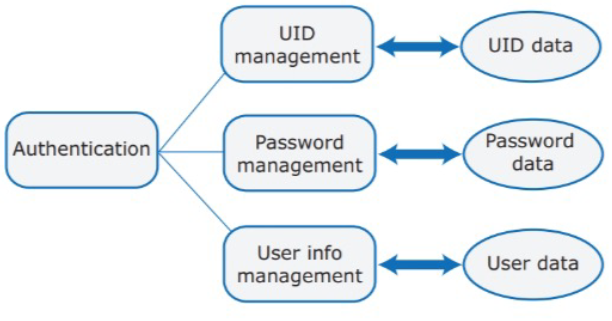
\includegraphics{images/microservices_auth.png}
      \caption{Result of microservices identification in our authentication example}
      \label{fig:microservices_auth}
   \end{figure}   
   \vspace{\fill}
\end{paracol}

\section{Microservices - Key Points}
\labelitemize{
   \textit{Microservices}
}{
   \begin{itemize}
      \item \textbf{Small-scale}\footnotemark services that can be combined to create applications
      \item \textbf{Independent}, i.e. service interface must not be affected by changes to other services
      \item Possible to modify and re-deploy service \textbf{without changing/stopping} other services
   \end{itemize}
}
\footnotetext{Actually sometimes they may be not so small}

More specifically, we can list more specific charateristics on how microservices should be:
\begin{itemize}
   \item \textit{Self-contained}
   \item \textit{Lightweight}
   \item \textit{Implementation independent}
   \item \textit{Independently deployable}
   \item \textit{Business-oriented}
\end{itemize}

When speaking of services "size" two measures come in handy:
\begin{enumerate}
   \item 
   \textbf{Coupling} measures number of \textit{inter}-component relationships.\\
   \textit{Low \textbf{coupling}} $\longrightarrow$ \textit{independent services, independent updates}\\
   Idea $\longrightarrow$ if two services interact too much, then they should have be unified in a single service.
   \item \textbf{Cohesion} measures number of \textit{intra}-component relationships.\\
   \textit{High \textbf{cohesion}} $\longrightarrow$ \textit{less inter-service communication overhead}\\
   idea $\longrightarrow$ if a service intracommunicates too much with itself, then it should be split into smaller services.
\end{enumerate}
The key principle which the two measures aim to address is the "Single responsibility principle",
which states that each service should do one thing only and should do it well.
\note{
   Responsibility $\neq$ single functional activity
}

Another way to determine how "big" should a microservice be is the \textit{"Rule of twos"}, stating that a Service can be developed, tested, and deployed in two weeks by a team which can be fed with two large pizzas (8-10 people).
May people are required for a single service for various reasons {---}e.g. developing, decoupling, testing, etc.{---} but
the most groundbreaking one is that \emph{services should be \textbf{supported} and maintained \textbf{after} deployment}

\section{Motivations}
\begin{enumerate}
   \item Accelerated rebuild and redeployment for \textbf{shorten lead time} for \textit{new features} and \textit{updates}
   \item \textbf{Scale}, effectively
\end{enumerate}

Microservices architecture perfectly assesses these two points, since each microservice can be deployed in a separate container, allowing for
quick \textbf{stop/restart} without affecting other services
and for quick deployment of service \textbf{replicas}.

\section{Design decisions}
\begin{figure}[htbp]
   \centering
   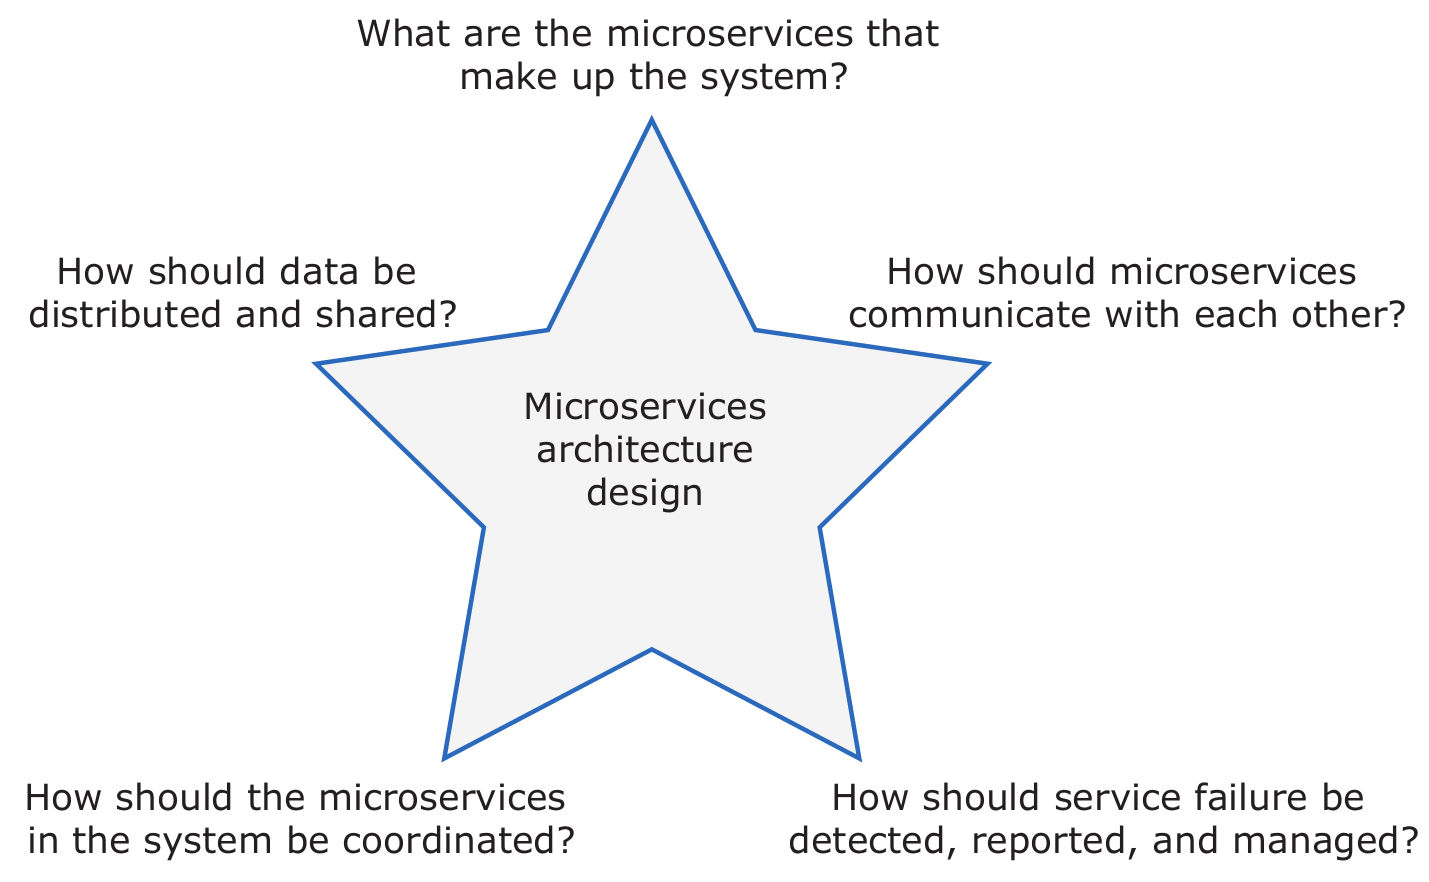
\includegraphics{images/microservices_decisions.png}
   \caption{Microservices Decisions}
   \label{fig:microservices_decisions}
\end{figure}

How to decompose system into a set of microservices?
They should be
not too many (low cohesion $\longrightarrow$ communication overhead) and also
not too few (high coupling $\longrightarrow$ less independency for updates/deployment/..)

Understanding how to decompose is not a trivial task:
\setlist[description]{itemsep=0em,topsep=0.5em,parsep=0em}
\setlist[itemize]{itemsep=0em}

\begin{itemize}[topsep=0em]
   \item Balance fine-grain functionality and system performance
   \item Follow the “common closure principle”
   (elements likely to be changed at the same time should stay in same service)
   \item Associate services with business capabilities
   \item Services should have access only the data they need
   (+ data propagation mechanisms)
\end{itemize}

\section{Service Communications}
\begin{figure}[htbp]
   \centering
   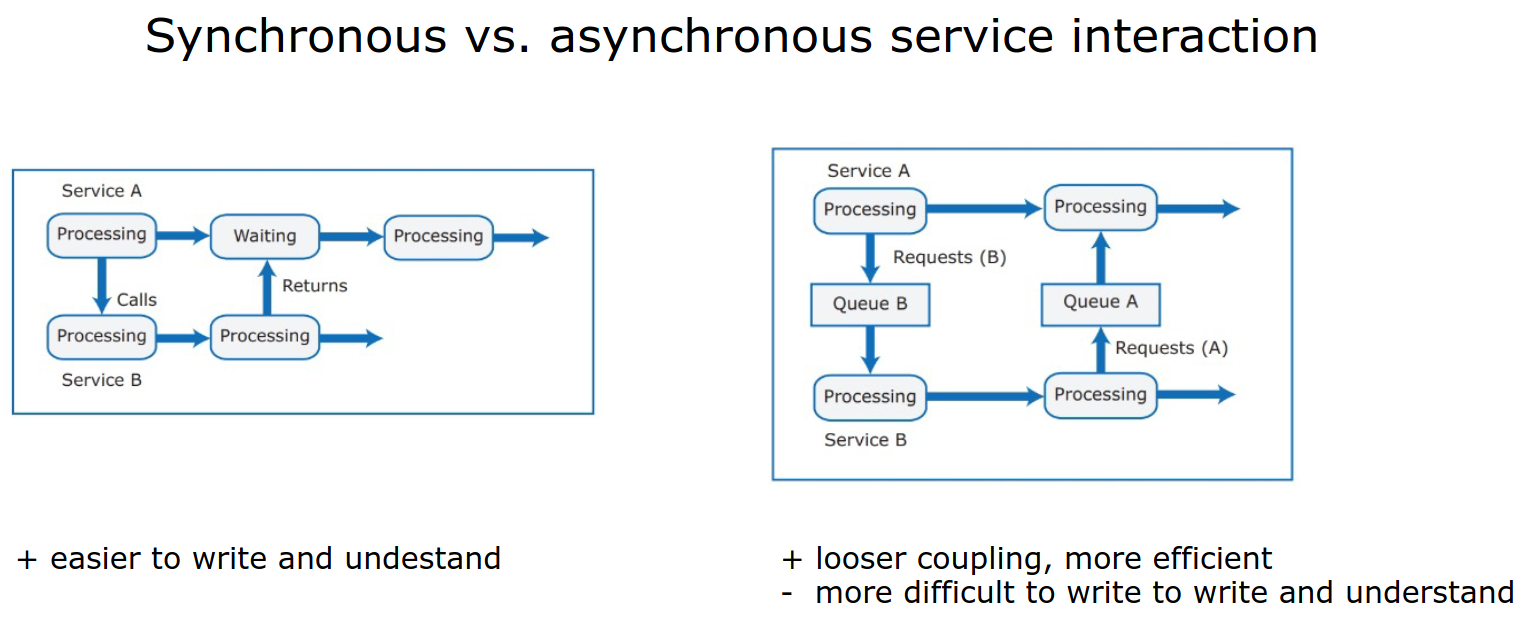
\includegraphics{images/microservices_communications1.png}\\
   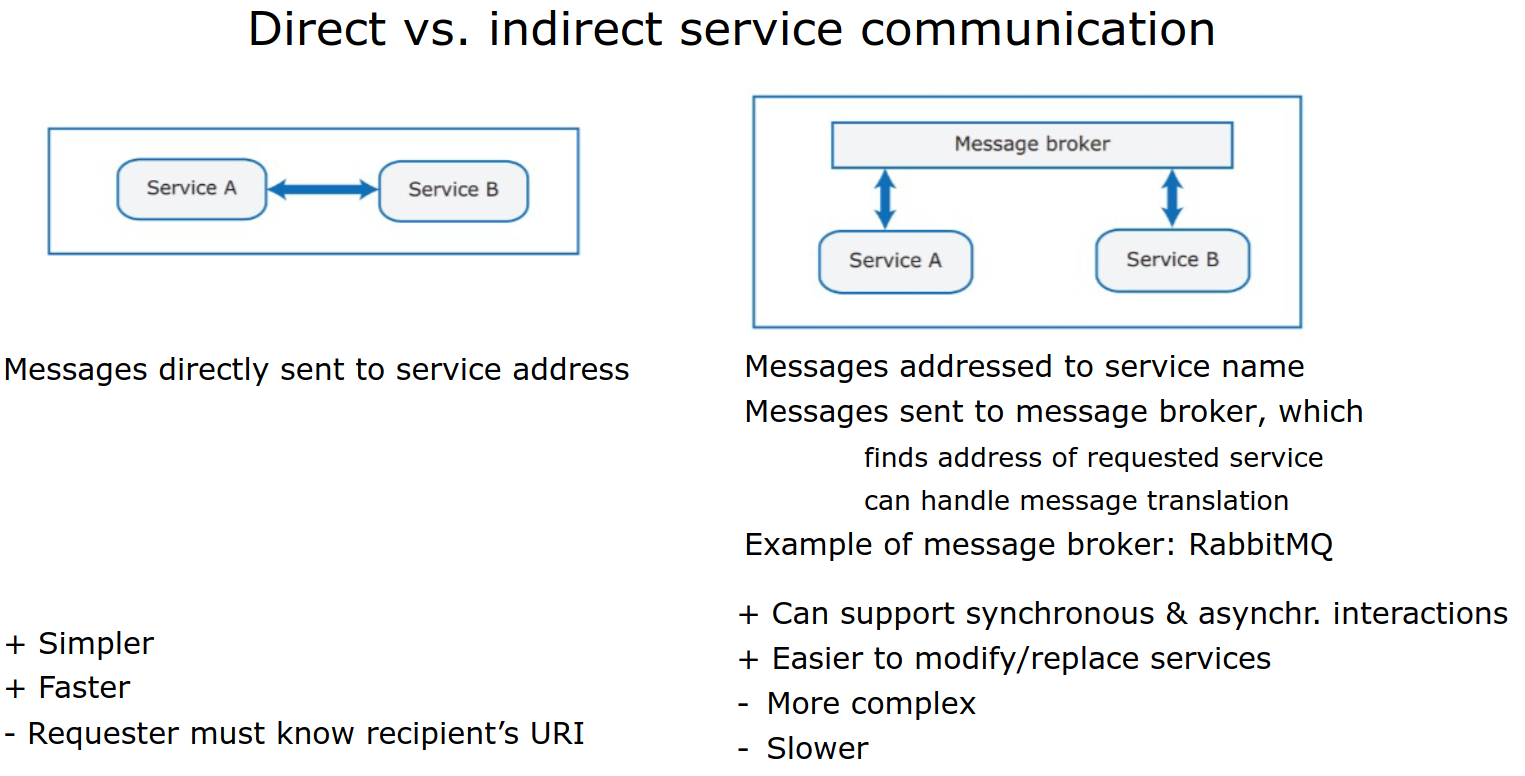
\includegraphics{images/microservices_communications2.png}
   \caption{Microservices communication}
   \label{fig:microservices_communications}
\end{figure}


Ideally each microservice should manage its \textit{own data}, but this arises the problem of dealing with possible \textbf{data dependencies}.\nl
To avoid major issues, data sharing should be as little as possible
and should mostly be \textit{read-only}, with few services responsible for data updates.
Besides, it is advisable to include a mechanism to keep \textbf{consistent db copies} used by replicated services.

Shared database architectures employ \texttt{ACID}\footnote{\textit{Atomicity Consistency Isolation Durability}} transactions to serialize updates and
avoid inconsistency.
In distributed systems we must trade-off data \textbf{consistency} and \textbf{performance},
hence microservices systems must be designed to \textbf{tolerate} some degree of data
\textbf{inconsistency}.
\begin{enumerate}
   \item \textit{Dependent data inconsistency}\\
   Actions/failures of one service can cause data managed by another service to become
   inconsistent
   \item \textit{Replica inconsistency}\\
   Several replicas of the same service may be executing concurrently,
   each one updating its own db copy.
   Thus, we need to make these dbs \textit{"eventually consistent"}\footnote{i.e."Sooner or later will be consistent", which is not "\textit{maybe} consistent \textit{maybe not}"}
\end{enumerate}

\subsection{CAP and Saga}
\begin{center}
   \textbf{\textit{CAP} Theorem}\\
   
   It is \textbf{impossible} for a web service to provide \textit{\underline{C}onsistency}, {\underline{A}vailability} and \textit{\underline{P}artition-tolerance}at the same time
   
   \note{
      In presence of a \textit{network \underline{P}artition}, you cannot have both \textit{\underline{A}vailability} and \textit{\underline{C}onsistency}
   }
\end{center}
\begin{enumerate}
   \item \textbf{Consistency}:
   any read operation that begins after a write operation must return that value, or the
   result of a later write operation
   \item \textbf{Availability}:
   every request received from a non-failing node must result in a response
   \item \textbf{Partition-tolerance}:
   services can be partitioned into multiple groups and network can delay lose arbitrarily many messages among services
\end{enumerate}

The \textbf{Saga pattern} provides a possible solution to handle consistency between transactions.

Implement each business transaction that spans between multiple services as a \textbf{saga}, i.e.
a sequence of local transactions.
Each local transaction updates a database and triggers next local transaction(s) in the saga;
in case such local transaction fails then the saga executes a series of \textbf{compensating transactions}.
\labelitemize{
   \textit{\textbf{Coordinating} sagas}
}{
   \begin{enumerate}
      \item \textit{Choreography}:
      each local transaction publishes event that triggers next local transaction(s)
      \item \textit{Orchestration}:
      an orchestrator tells participants which local transactions to execute
   \end{enumerate}
}

\labelitemize{
   \textit{\textbf{Coordinating} sagas}
}{
   \begin{enumerate}
      \item \textit{Backward model}: \textbf{undo} changes made by previously executed local transactions
      \item \textit{Forward model}: "\textbf{retry} later"
   \end{enumerate}
}

\subsection{Netflix Approach}

Netflix eventual consistency is backed up by \textit{Apache Cassandra},
in a nutshell, to replicate data in n nodes:
"write to the ones you can get to, then fix it up afterwards";
A quorum is used as threshold, e.g. $(n/2 + 1)$ of the replicas must respond.

\begin{figure}[htbp]
   \centering
   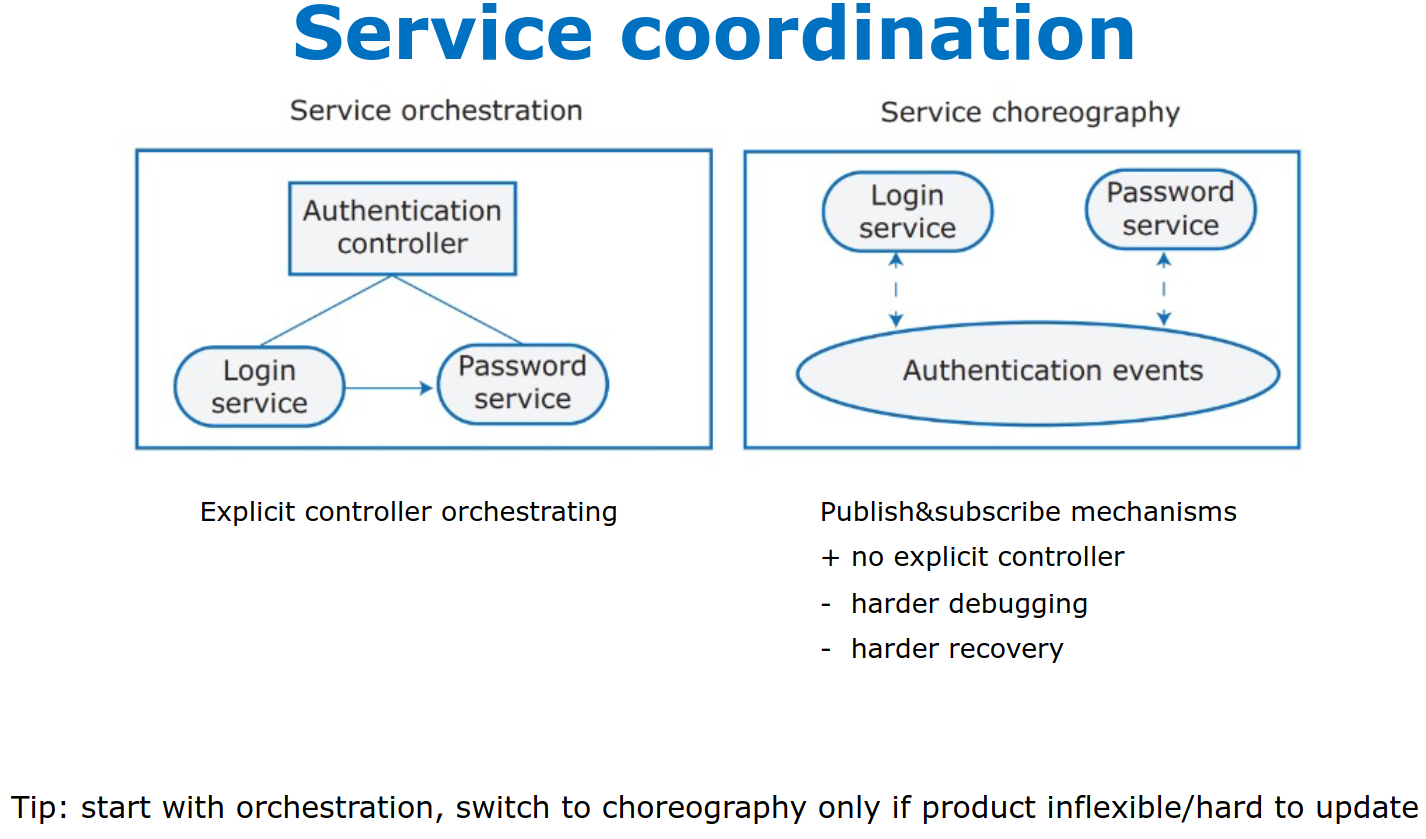
\includegraphics{images/netflix_coordination.png}
   \caption{Netflix approach on Coordination}
   \label{fig:netflix_coordination}
\end{figure}

\subsection{Failure management}

\begin{paracol}{2}
   \vspace{\fill}
   
   Something will \textbf{unavoidably} go wrong,
   regardless of everything.
   A system must be able to cope with failures.
   \nl

   Consider for instance a service $S$ invoking two other services $A$ and $B$ which guarantee $99\%$ availability, then:
   \[
      downtime(S) = 30\frac{min}{\textbf{day}}
   \]

   \note{30 minutes per day of \textbf{downtime} is a lot!}

   \vspace{\fill}

   \switchcolumn

   \begin{enumerate}
      \item \textbf{Internal} failure:
      Conditions detected by a service and which can be reported to the \textit{requestor} service through an error message for instance.\\
      e.g. invalid link/resource not found.  
      \item \textbf{External} failure:
      External cause which affects the availability of a service,
      possibly leading to its unresponsiveness.
      \item \textbf{Performance} failure:
      Performance has degregated to an unacceptable level.
   \end{enumerate}
\end{paracol}

\begin{figure}[htbp]
   \centering
   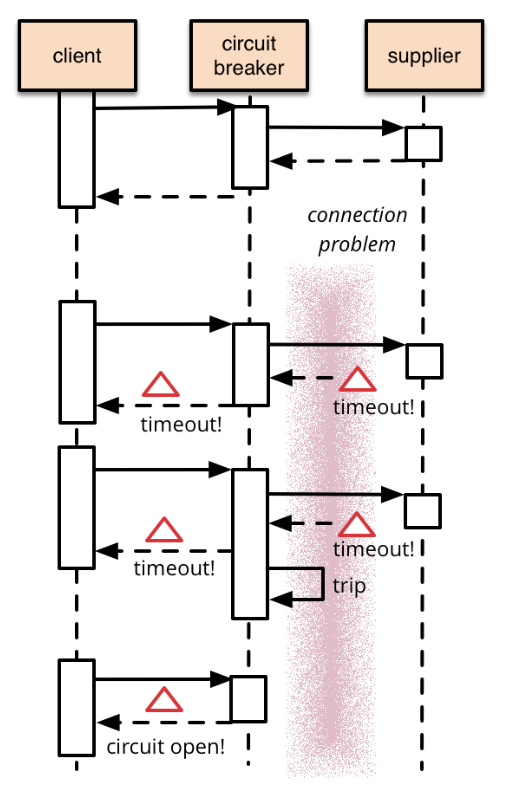
\includegraphics[width=0.2\columnwidth]{images/circuit_breaker.png}
   \caption{Circuit breaker}
   \label{fig:circuit_breaker}
\end{figure}
One way to cope with failures is to exploit \textbf{Circuit breakers} (Fig \ref{fig:circuit_breaker}),
which are based on timeouts to compensate unresponsiveness of a requested service.\\
Another way is to "bravely" test using the \textbf{Chaos Monkey} paradigm,
which causes at a given rate random failures in the tested system.

\newpage
\section{RESTful services}
\begin{paracol}{2}
   \textit{\underline{RE}presentational \underline{S}tate \underline{T}ransfer} (\textbf{REST}) was originally introduced as an architectural
   style, 
   and then it has developed as an abstract model of the
   Web architecture to guide the redesign and
   definition of HTTP and URIs.
   
   \switchcolumn

   \begin{center}
      \textit{
      "each action resulting in a transition
      to the next state of the application by
      transferring a representation of that
      state to the user"}
   \end{center}

\end{paracol}

\labelitemize{
   \textit{\textbf{REST} principles}
}{
   \begin{enumerate}
      \item \textit{Resource identification through URIs}:
            \begin{enumerate}
               \item Service exposes set of resources identified by \texttt{URI}s
            \end{enumerate}
      \item \textit{Uniform interface}:
            \begin{enumerate}
               \item Clients invoke \texttt{HTTP} methods to \textit{create/read/update/delete} resources:
               \item \texttt{POST} and \texttt{PUT} to create and update state of resource
               \item \texttt{DELETE} to delete a resource
               \item \texttt{GET} to retrieve current state of a resource
            \end{enumerate}
      \item \textit{Self-descriptive messages}:
            \begin{enumerate}
               \item Requests contain enough context information to process message
               \item Resources decoupled from their representation so that content can be accessed in a
               variety of formats (e.g., \texttt{HTML}, \texttt{XML}, \texttt{JSON}, \texttt{plain  text}, \texttt{PDF}, \texttt{JPEG}, etc.)
            \end{enumerate}
      \item \textit{Stateful interactions through hyperlinks}:
            \begin{enumerate}
               \item Every interaction with a resource is stateless
               \item Server contains no client state, any session state is held on the client
               \item Stateful interactions rely on the concept of explicit state transfer
            \end{enumerate}
         \end{enumerate}
}

\section{DevOps}

\begin{figure}[htbp]
   \centering
   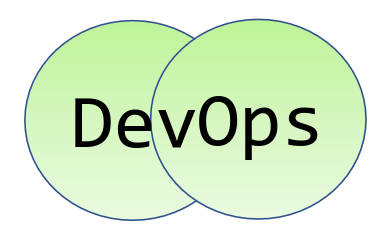
\includegraphics[width=0.2\columnwidth]{images/devops.png}
   \label{fig:devops}
\end{figure}
\begin{center}
   Same team responsible for service\\
   \textbf{development}, \textbf{deployment} and \textbf{managements}.
\end{center}

\begin{figure}[htbp]
   \centering
   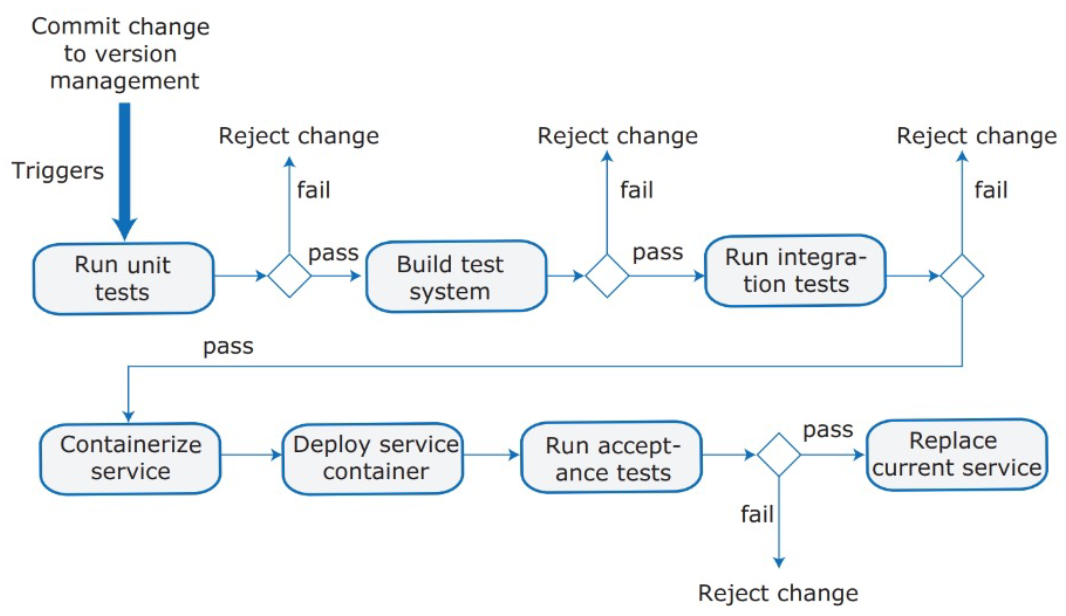
\includegraphics{images/devops_pipeline.png}
   \caption{Continuous deployment pipeline}
   \label{fig:devops_pipeline}
\end{figure}

However, regardless of how intense it is, testing \textit{cannot} prevent 100\% of unanticipated problems,
thus it is mandatory to \textbf{monitor} the deployed services.
Heavy monitoring may affect the performance of services and the overall usability of a product,
thus it must be sufficient to meet our needs and not more.\\
Monitoring allows to detect the failure of a service and \textbf{rollback} if needed.
When introducing a \textit{new} version of a service, you maintain the \textit{old} version,
changing only the "current version link" to point at the new service,
remaining able to revert it if needed.

\section{Concluding Remarks}
\begin{paracol}{2}
   \vspace{\fill}
   \labelitemize{
      \color{darkgreen}
      \textit{Microservices - Pros}
   }{
      \color{darkgreen}
      \begin{itemize}
         \item Shorter lead time
         \item Effective scaling
      \end{itemize}
   }
   \vspace{\fill}
   \switchcolumn
   
   \labelitemize{
      \color{darkred}
      \textit{Microservices - Cons}
   }{
      \begin{itemize}
         \color{darkred}
         \item Communication overhead
         \item Complexity
         \item "Wrong cuts"
         \item "Avoiding data duplication as much as possible while keeping microservices in isolation
         is one of the biggest challenges"
      \end{itemize}
   
      \hspace{1em}"A poor team will always create a poor system"
   }
\end{paracol}

\begin{figure}[htbp]
   \centering
   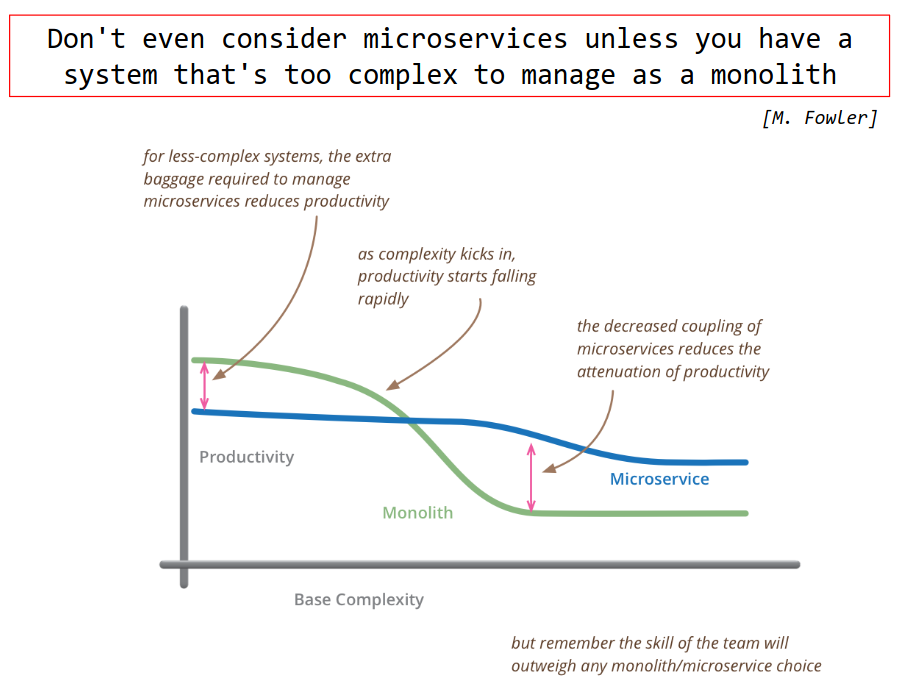
\includegraphics{images/microservices_takeaway.png}
   \caption{Takeaway message}
   \label{fig:microservices_takeaway}
\end{figure}